\section{Introduction}\label{sec:intro}
zbMATH classified more than 
\href{https://zbmath.org/?q=%2A+py%3A2019}%
{80k} articles in 2019 according to the Mathematical Subject Classification~(MSC).
With more than
\href{https://msc2020.org}%
{5000} class labels, this classification task requires significant depth-knowledge of the particular fields of mathematics in order to obtain correct fine-grained classifications of the articles.
Therefore the classification is two-fold.
At first, the articles are pre-classified into one of \href{https://msc2020.org}%
{63} main classifications, which are the two first digits of the first MSC label of each article.
In a second step, domain expert assigns fine-grained classification labels in their area of expertise.

In this paper, we focus on the coarse-grained classification and explore how modern machine learning technology can be employed to automate this process.
In particular, we compare the current state of the art technology with a system customized for the application in zbMATH from 2014~\cite{SchonebergS14}. 
We formulate the following research questions:
\begin{enumerate}
  \item Which measures are appropriate to measure the quality of automatic classifications?
  \item Does the inclusion of mathematical formulae improve the quality of the classifications?
  \item Does the Part of Speech (POS) preprocessing improve the quality of classifications?
  \item Which features (Title, Abstract, References) are most important for the correct classification?
  \item How does the quality of automatic classification compare to manual classifications?
  \item How to avoid misclassifications in the future?
  \item How can the best performing method be integrated into the current production pipeline at zbMATH?
\end{enumerate}
\section{Method}\label{sec:method}
To investiagte the given problem, we first create a test and training dataset, second we investage different encodings, train our models and evaluate the results.
\subsection{Generation of a test and training dataset}
\subsection{Definition of evaluation metrics}
\subsection{Encoding of the input data}
\subsection{Clustering}
\subsection{Reproducibility}
\url{https://mathscinet.ams.org/mathscinet-getitem?mr=3444005}

\section{Evaluation}\label{sec:eval}

\subsection{pre-Evaluation}
\begin{figure}[h]
  \centering
  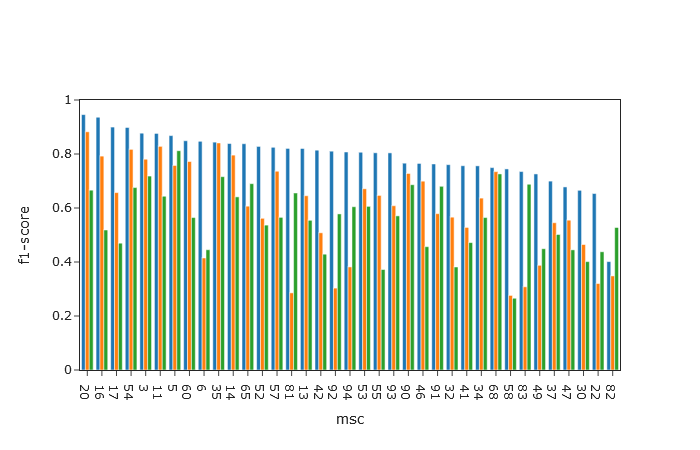
\includegraphics[width=1.1\textwidth]{zbMr.png}
  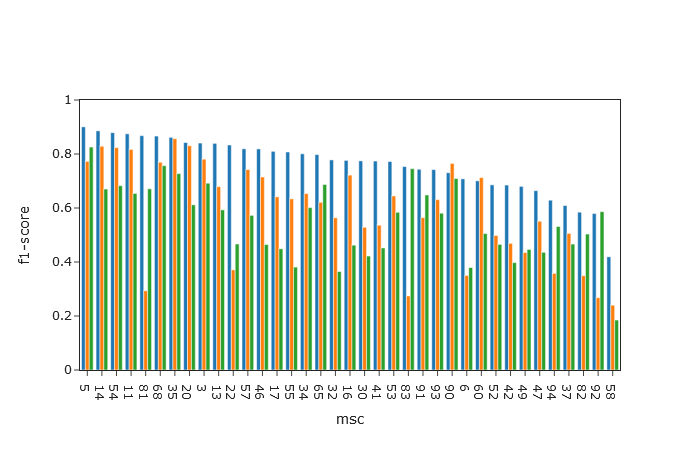
\includegraphics[width=1.1\textwidth]{mrZb.png}
  \caption{$F_1$ score of the classification quality of the (other Institution, MSCbR alorith, and the S14 algoritm) grouped by MSC. The top figure uses the zbMATH primary MSC as baseline and the bottom figure uses the MR primary MSC respectively. MSC classes with less than 200 samples were omitted. }
\end{figure}


\begin{table*}
\begin{tabular}{llll}
  \toprule
  {} &      p &      r &      f \\
  \midrule
  zb1   &      1 &      1 &      1 \\
  mr1   &  0.814 &  0.814 &  0.812 \\
  titer &  0.772 &  0.778 &  0.773 \\
  refs  &  0.748 &  0.753 &  0.746 \\
  titls &  0.637 &  0.627 &  0.623 \\
  texts &  0.699 &  0.709 &  0.699 \\
  ref1  &  0.693 &  0.648 &  0.652 \\
  uT1   &  0.656 &  0.642 &  0.645 \\
  uM1   &  0.655 &  0.639 &  0.644 \\
  tiref &   0.76 &  0.764 &   0.76 \\
  teref &  0.769 &  0.774 &   0.77 \\
  tite  &  0.713 &  0.722 &  0.713 \\
  \bottomrule
\end{tabular}
\begin{tabular}{llll}
  \toprule
  {} &      p &      r &      f \\
  \midrule
  zb1   &  0.817 &  0.807 &   0.81 \\
  mr1   &      1 &      1 &      1 \\
  titer &  0.776 &  0.775 &  0.772 \\
  refs  &  0.743 &  0.743 &  0.737 \\
  titls &  0.644 &  0.632 &  0.627 \\
  texts &  0.704 &  0.709 &  0.699 \\
  ref1  &  0.693 &  0.646 &  0.652 \\
  uT1   &  0.653 &  0.636 &  0.639 \\
  uM1   &  0.652 &  0.632 &  0.636 \\
  tiref &  0.762 &  0.761 &  0.758 \\
  teref &  0.771 &   0.77 &  0.767 \\
  tite  &   0.72 &  0.724 &  0.715 \\
  \bottomrule
\end{tabular}
\caption{Precision $p$, recall $r$ and $F_1$-measure $f$ with regard to the baseline zb1 (left) and mr1 (right).}
\end{table*}


\section{Conclusion \& Future Work}\label{sec.concl}
Regarding the research questions, we summarize our findings as follows:
\begin{enumerate}
  \item The quality of the classification for the coarse grained primary MSC can be evaluated with classical information retrieval methods such as precision, recall and accuracy. The downside of binary evaluation approaches is that the degree of incorrectness is not taken into account. We therefore introduced a non-strict evaluation measure that also counts non-primary MSCs as correct.
  \item We did not find evidence that mathematical expressions improve the coarse grained primary classification.
  \item We found that modern NN such as Bert outperform the POS tagging based model developed by \cite{SchonebergS14}. mathematical expressions improve the coarse grained primary classification.
  \item For most classes the reference based approach outperformed the POS tagged based approach.
  \item The manual classification is significantly better for most classes. 
  \item How to avoid misclassifications in the future?
  \item How can the best performing method be integrated into the current production pipeline at zbMATH?
\end{enumerate}

\paragraph{Acknowledgments} This work was supported by the German Research Foundation (DFG grant GI 1259-1).
The authors would like to express their gratitude to Felix Hamborg, and Terry Ruas for their advice in the most recent machine learning technology.
\printbibliography[keyword=primary]